%-------------------------------------------------------------------------------
%                                PREAMBLE
%-------------------------------------------------------------------------------
\documentclass[usenames,dvipsnames,svgnames,10pt,aspectratio=169]{beamer}
\usefonttheme{professionalfonts}

% This theme uses TIKZ: compile twice with PDFLaTeX or LuaLaTeX.
%
%  Options:
%  - [clean]:    clean slides, i.e. logos and footbar are removed
%  - [kth]:      footbar style inspierd to the official KTH template
%  - [nicewave]: a different style of wave is used (not approved by FLOW)
%
\usetheme{flow}

\usepackage{hyperref,graphicx,lmodern}
\usepackage[utf8]{inputenc}
\usepackage{media9}
\usepackage{xcolor}
\usepackage{stmaryrd}
\usepackage{nicefrac}
\usepackage{multimedia}
\usepackage{multicol}
\usepackage{upgreek}
\usepackage[]{bm}
\usepackage[]{url}

\DeclareMathOperator{\sinc}{sinc}
\DeclareMathAlphabet{\mathcal}{OMS}{cmsy}{m}{n}
\DeclareMathAlphabet\mathbfcal{OMS}{cmsy}{b}{n}

\graphicspath{{imgs/}}
\setbeamertemplate{blocks}[rounded][shadow=true]

\DeclareMathOperator{\trace}{tr}

%-------------------------------------------------------------------------------
%                                TITLE PAGE
%-------------------------------------------------------------------------------
\title[Nonlinear Physics] % Short title used in footline
{
	Nonlinear physics, dynamical \\ systems and chaos theory
}

\author[J.-Ch.~Loiseau] % Presenting author in short form used in footline
{
	Jean-Christophe Loiseau
}
% - Give the names in the same order as the appear in the paper.
% - Underline the presenting author.

\institute[unused]
{
	\url{jean-christophe.loiseau@ensam.eu} \\
	DynFluid, \\
	Arts et M\'etiers ParisTech, France
}
% Keep it simple, no one is interested in your street address.

% University logo(s)
\logot{
\includegraphics[width=.128\paperwidth]{DynFluid_logo}}  % Top logo
\logob{
\includegraphics[width=0.128\paperwidth]{ENSAM_logo}} % Bottom logo
% \logoc[{
\includegraphics[width=.128\paperwidth]{limsi}}]{
\includegraphics[width=.128\paperwidth]{limsi}} % Corner logo
%
% Cover image: \cvrimg{x position}{y position}{cover image}
\cvrimg{.77}{.8}{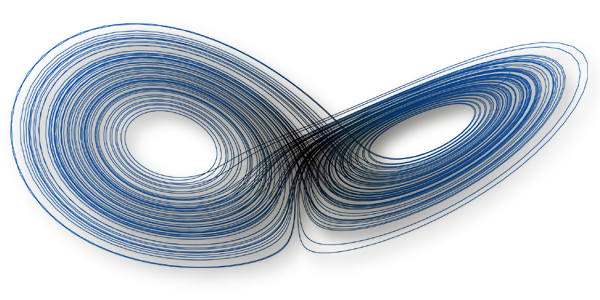
\includegraphics[width=.4\paperwidth]{cover.png}}

\date[unused]{ENSAM, Master 2, 2018--2019}

\begin{document}

\titleframe % Print the title as the first slide

%-------------------------------------------------------------------------------
%                           PRESENTATION SLIDES
%-------------------------------------------------------------------------------

\begin{frame}[t, c]{}
	\centering
	\vspace{1cm}

	{\Large \textbf{Rayleigh-Bénard convection}}

	\bigskip

	{\textgre{\textbf{Context and governing equations}}}

\end{frame}

\begin{frame}[t, c]{Rayleigh-Bénard convection}{Overview}
	\begin{minipage}{.48\textwidth}
		\begin{itemize}
			\item Buoyancy-driven flow of a fluid heated from below and cooled from above.

			\medskip

			\item Applications in geophysics, astrophysics, meteorology, oceanography and engineering.

			\medskip

			\item Well-known model for nonlinear and chaotic dynamics, pattern formation and fully developed turbulence.
		\end{itemize}
	\end{minipage}%
	\hfill
	\begin{minipage}{.48\textwidth}
		\centering
		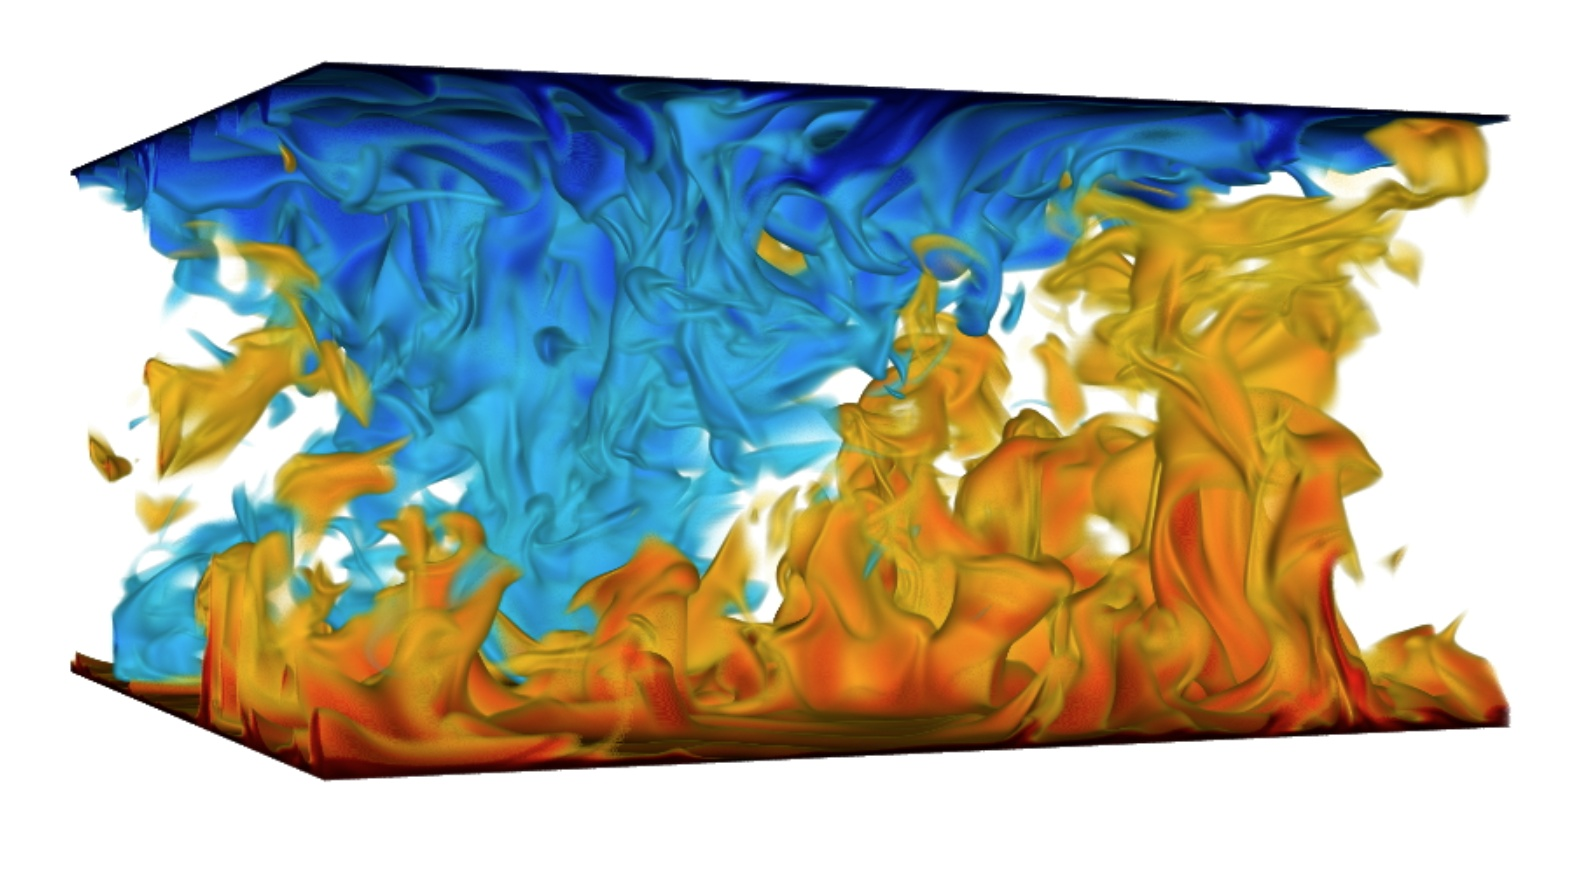
\includegraphics[width=.95\textwidth]{turbulent_rayleigh_benard} \\

		{\small Illustration of turbulent Rayleigh-Bénard convection.}
	\end{minipage}

	\vspace{1cm}
\end{frame}

\begin{frame}[t, c]{Rayleigh-Bénard convection}{Driving force: Buoyancy}
	\begin{block}{\centering \textbf{Archimedes' principle} (c. 250 BC)}
		\centering
		\begin{quote}
			Any object, wholly or partially immersed in a stationary fluid, is buoyed up by a force equal to the weight of the fluid displaced by the object.
		\end{quote}
	\end{block}

	\bigskip

	\begin{itemize}
		\item This force is modeled as
		\begin{equation}
			\overrightarrow{\pi} = - \rho_f V_f \overrightarrow{g}
			\notag
		\end{equation}
		where $\rho_f$ is the fluid's density, $V_f$ is the volume of fluid displaced by the object and $\overrightarrow{g}$ is gravitational acceleration.
	\end{itemize}

	\vspace{1cm}
\end{frame}

\begin{frame}[t, c]{Rayleigh-Bénard convection}{Density and temperature}
	\begin{itemize}
		\item Assuming an incompressible flow, the state equation can be approximated as
		\begin{equation}
			\rho = \rho_0 \left( 1 - \alpha (T - T_0) \right)
			\notag
		\end{equation}
		where $\alpha$ is the coefficient of thermal expansion.

		\bigskip

		\item This approximation is known as \alert{\textbf{Boussinesq approximation}}.
	\end{itemize}

	\vspace{1cm}
\end{frame}

\begin{frame}[t, c]{Rayleigh-Bénard convection}{Governing equations}
	\begin{itemize}
		\item The flow is governed by
		\begin{equation}
			\begin{aligned}
				\nabla \cdot \bm{u} & = 0 \\
				\displaystyle \frac{\partial \bm{u}}{\partial t} + \left( \bm{u} \cdot \nabla \right) \bm{u} & = - \frac{1}{\rho} \nabla p + \nu \nabla^2 \bm{u} + \delta \rho \bm{g} \\
				\displaystyle \frac{\partial T}{\partial t} + \left( \bm{u} \cdot \nabla \right) T & = \kappa \nabla^2 T,
			\end{aligned}
			\notag
		\end{equation}
		where $\bm{u}$ is the fluid's velocity, $\rho$ its density and $T$ is the temperature. $\nu$ and $\kappa$ are the kinematic viscosity and the thermal diffusivity, respectively.
	\end{itemize}

	\vspace{1cm}
\end{frame}

\begin{frame}[t, c]{Rayleigh-Bénard convection}{Nondimensional form}
	\begin{itemize}
		\item Under appropriate nondimensionalization, the governing equations read
		\begin{equation}
			\begin{aligned}
				\nabla \cdot \bm{u} & = 0 \\
				\displaystyle \frac{\partial \bm{u}}{\partial t} + \left( \bm{u} \cdot \nabla \right) \bm{u} & = - \nabla p + Pr \nabla^2 \bm{u} + \left( Ra\ Pr \right) \theta \bm{e}_y \\
				\displaystyle \frac{\partial \theta}{\partial t} + \left( \bm{u} \cdot \nabla \right) \theta & = \nabla^2 \theta,
			\end{aligned}
			\notag
		\end{equation}
		where $Pr$ is the Prandtl number and $Ra$ the Rayleight number. $\theta$ is the nondimensional temperature given by $\theta = \nicefrac{T-T_c}{T_h - T_c}$.
	\end{itemize}

	\vspace{1cm}
\end{frame}

\begin{frame}[t, c]{}
	\centering
	\vspace{1cm}

	{\Large \textbf{Rayleigh-Bénard convection}}

	\bigskip

	{\textgre{\textbf{Base state and linear stability analysis}}}

\end{frame}

\begin{frame}[t, c]{Rayleigh-Bénard convection}{Fixed point: the conducting state}
	\begin{itemize}
		\item The fixed point is solution to
		\begin{equation}
			\displaystyle \frac{\mathrm{d}^2 \Theta}{\mathrm{d}y^2} = 0
			\notag
		\end{equation}
		with appropriate boundary conditions.

		\bigskip

		\item The nondimensional temperature profile $\Theta(y)$ is solution to the heat equation. It is given by
		$$\Theta (y) = 1 -y.$$

		\bigskip

		\item It corresponds to a pure conduction state (i.e.\ $\bm{u} = 0$).
	\end{itemize}

	\vspace{1cm}
\end{frame}

\begin{frame}[t, c]{Rayleigh-Bénard convection}{Linear stability analysis}
	\begin{itemize}
		\item Let us consider the linear stability of this conducting state towards two-dimensional perturbations (see Squire theorem).

		\bigskip

		\item The linearized equations read
		\begin{equation}
			\begin{aligned}
				\displaystyle \frac{\partial}{\partial t} \nabla^2 \psi & = - Ra\ Pr \frac{\partial \theta}{\partial x} +  Pr \nabla^2 \psi \\
				\displaystyle \frac{\partial \theta}{\partial t} & = - \frac{\partial \psi}{\partial x} + \nabla^2 \theta,
			\end{aligned}
			\notag
		\end{equation}
		where $\psi$ is the streamfunction of the perturbation.
	\end{itemize}

	\vspace{1cm}
\end{frame}

\begin{frame}[t, c]{Rayleigh-Bénard convection}{Linear stability analysis}
	\begin{itemize}
		\item Solutions are sought in the form of \emph{normal modes}, i.e.\
		$$\bm{q}(x, y, t) = \hat{\bm{q}}(y) e^{ikx + \lambda t} + \mathrm{c.c},$$
		where $\lambda$ is the growth rate and $k$ the perturbation's wavenumber.

		\bigskip

		\item We obtain the following generalized eigenvalue problem
		\begin{equation}
			\lambda
			\begin{bmatrix}
				D^2 - k^2 & 0 \\
				0 & 1
			\end{bmatrix}
			\begin{bmatrix}
				\hat{\psi} \\
				\hat{\theta}
			\end{bmatrix}
			=
			\begin{bmatrix}
				Pr (D^2 - k^2) & -ik Ra\ Pr \\
				-ik & D^2-k^2
			\end{bmatrix}
			\begin{bmatrix}
				\hat{\psi} \\
				\hat{\theta}
			\end{bmatrix}
			\notag
		\end{equation}
		where $D = \nicefrac{\mathrm{d}}{\mathrm{d}y}$.
	\end{itemize}

	\vspace{1cm}
\end{frame}

\begin{frame}[t, c]{Rayleigh-Bénard convection}{Linear stability analysis}
	\begin{minipage}{.64\textwidth}
		\begin{itemize}
			\item This problem has been solved analytically in 1916, assuming free-slip boundary conditions, i.e.\
			\begin{equation}
				\begin{aligned}
					\psi(x, y, t) & = \hat{\psi}(t) \sin (n \pi y) \sin(kx)\\
					\theta(x, y, t) & = \hat{\theta}(t) \sin (n \pi y) \cos(kx).
				\end{aligned}
				\notag
			\end{equation}

			\bigskip

			\item The dispersion relation reduces to a quadratic equation. One then obtains $Ra_c = \nicefrac{27 \pi^4}{4}$ and $k_c = \nicefrac{\pi}{\sqrt{2}}$.
		\end{itemize}
	\end{minipage}%
	\hfill
	\begin{minipage}{.32\textwidth}
		\centering
		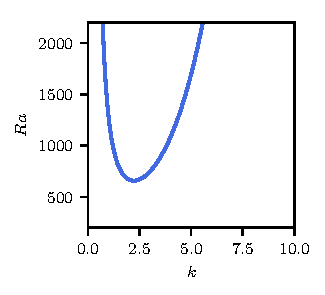
\includegraphics[width=.9\textwidth]{rayleigh_benard_dispersion_relation}
	\end{minipage}

	\vspace{1cm}
\end{frame}

\begin{frame}[t, c]{Rayleigh-Bénard convection}{Linear stability analysis}
	\centering
	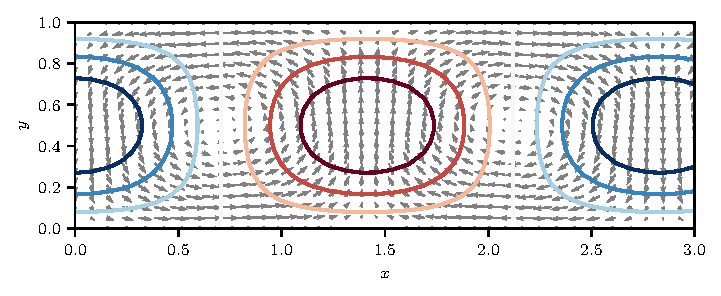
\includegraphics[width=.75\textwidth]{rayleigh_benard_instability_mode}

	Isocontours of temperature and velocity field of the instability mode.

	\vspace{1cm}
\end{frame}

\begin{frame}[t, c]{}
	\centering
	\vspace{1cm}

	{\Large \textbf{From Navier-Stokes to Lorenz}}

	\bigskip

	{\textgre{\textbf{Investigating the nonlinearities}}}

\end{frame}

\begin{frame}[t, c]{From Navier-Stokes to Lorenz}{Nonlinear equations}
	\begin{itemize}
		\item The governing equations read
		\begin{equation}
			\begin{aligned}
				& \displaystyle \frac{\partial}{\partial t}\nabla^2 \psi - Pr \nabla^2 \psi + (Ra\ Pr)\frac{\partial \theta}{\partial x} = \mathcal{J} \left( \nabla^2 \psi, \psi \right) \\
				& \displaystyle \frac{\partial \theta}{\partial t} - \nabla^2 \theta + \frac{\partial \psi}{\partial x} = \mathcal{J}\left( \theta, \psi \right),
			\end{aligned}
			\notag
		\end{equation}
		where the nonlinear terms are expressed as a Jacobian operator $\mathcal{J}$ given by
		$$\mathcal{J}(f, g) = \displaystyle \frac{\partial f}{\partial x}\frac{\partial g}{\partial y} - \frac{\partial g}{\partial x}\frac{\partial f}{\partial y}.$$

		\item We futhermore assume free-slip boundary conditions as before.
	\end{itemize}

	\vspace{1cm}
\end{frame}

\begin{frame}[t, c]{From Navier-Stokes to Lorenz}{Truncated Galerkin expansion}
	\begin{itemize}
		\item It has been shown by Saltzmann (1962) that the general solution can be expressed as an infinite Fourier series.

		\bigskip

		\item Let us however consider a \emph{truncated Galerkin expansion} such that
		\begin{equation}
			\begin{aligned}
				\psi(x, y, t) & = a(t) \sin(\pi y) \sin(k \pi x) + \cdots \\
				\theta(x, y, t) & = b(t) \sin(\pi y) \cos(k \pi x) + c(t) \sin(2 \pi y) + \cdots
			\end{aligned}
			\notag
		\end{equation}

		\bigskip

		\item $a(t)$ and $b(t)$ correspond to the convection rolls with wavenumber $k$ in the $x$-direction. The term $c(t)$ describes the modification of the mean temperature profile due to convection.
	\end{itemize}

	\vspace{1cm}
\end{frame}

\begin{frame}[t, c]{From Navier-Stokes to Lorenz}{Derivation of the low-order model}
	\centering
	It is now up to you to derive the low-order model :)

	\vspace{1cm}
\end{frame}

\begin{frame}[t, c]{From Navier-Stokes to Lorenz}{Low-order model}
	\begin{itemize}
		\item Finally, we obtain the following low-order model
		\begin{equation}
			\begin{aligned}
				\displaystyle \frac{\mathrm{d}a}{\mathrm{d}t} & = -\mathrm{Pr}\ \pi^2 (1+k^2)a - \frac{k \pi}{\pi^2(1+k^2)} \mathrm{Pr}\ \mathrm{Ra}\ b\\
				\displaystyle \frac{\mathrm{d}b}{\mathrm{d}t} & = -k \pi a - \pi^2(1+k^2)b - k\pi^2 a c \\
				\displaystyle \frac{\mathrm{d}c}{\mathrm{d}t} & = \displaystyle \frac{1}{2} k \pi^2 ab - 4\pi^2 c.
			\end{aligned}
			\notag
		\end{equation}

		\medskip

		\item This low-dimensional model of thermal convection is a rescaled version of the one originally introduced by Lorenz in 1963.
	\end{itemize}

	\vspace{1cm}
\end{frame}

\begin{frame}[t, c]{}
	\centering
	\vspace{1cm}

	{\Large \textbf{Lorenz system}}

	\bigskip

	{\textgre{\textbf{An example of chaotic dynamics}}}

\end{frame}

\begin{frame}[t, c]{Lorenz system}{1963 model}
	\begin{itemize}
		\item Lorenz-1963 model reads
		\begin{equation}
			\begin{aligned}
				\dot{x} & = \sigma ( y - x ) \\
				\dot{y} & = x ( \rho - z ) - y \\
				\dot{z} & = xy - \beta z,
			\end{aligned}
			\notag
		\end{equation}
		where $\sigma = Pr$, $\rho = \nicefrac{Ra}{Ra_c}$ and $\beta = \nicefrac{2\pi^2}{\pi^2+k^2}$ is the aspect ratio of the convection cells.

		\bigskip

		\item We consider the same parameters as Lorenz, i.e.\ $\sigma = 10$ (water) and $\beta = \nicefrac{8}{3}$.
	\end{itemize}

	\vspace{1cm}
\end{frame}

\begin{frame}[t, c]{Lorenz system}{Properties}
	\begin{itemize}
		\item \alert{\textbf{Symmetry}}: Invariant to the transformation $(x, y, z) \to (-x, -y, z)$.

		\bigskip

		\item \alert{\textbf{Invariant z-axis}}: If $x(0) = y(0) = 0$, then $x(t) = y(t) = 0 \ \forall t$. Then $\dot{z} = - \beta z$ and hence $z(t) = e^{-\beta z}$. The $z$-axis is thus always part of the stable manifold for the equilibrium at the origin.

		\bigskip

		\item \alert{\textbf{Dissipative}}: We have $\nabla \cdot \mathbfcal{F}(\mathbf{x}) = - \sigma - 1 - \beta < 0$. Any given volume $V$ of phase points will eventually tend to $0$ as $t \to \infty$.
	\end{itemize}

	\vspace{1cm}
\end{frame}

\begin{frame}[t, c]{Lorenz system}{Primary bifurcation}
	\begin{enumerate}
		\item Compute the fixed points of the system as a function of $\rho$.
		\item When does the conduction state (i.e.\ $\bm{x}^* = 0$) loose its stability?
		\item Are the resulting fixed points linearly stable or not? Conclude about the type of bifurcation encountered.
	\end{enumerate}

	\vspace{1cm}
\end{frame}

\begin{frame}[t, c]{Lorenz system}{Dynamics for $1 \leq \rho \leq 14$}
	\centering
	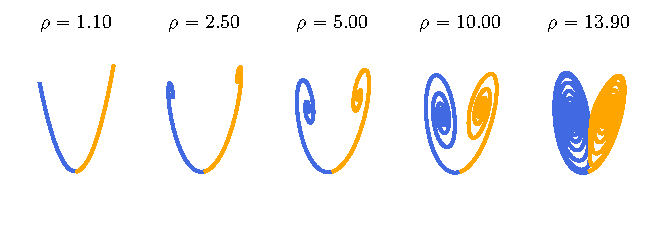
\includegraphics[width=.8\textwidth]{primary_bifurcation_phase_plots}

	\vspace{1cm}
\end{frame}

\begin{frame}[t, c]{Lorenz system}{Homoclinic connection ($\rho \simeq 13.926$)}
	\begin{minipage}{.48\textwidth}
		\begin{itemize}
			\item Existence of a homoclinic connection for $\rho \simeq 13.926$.
			\begin{itemize}
				\item[$\hookrightarrow$] Perturbation leaves the conducting state along its unstable manifold and returns to it along its stable one.
			\end{itemize}

			\bigskip

			\item For $\rho > 14$, the system exhibits \emph{pre-chaotic} transients.
		\end{itemize}
	\end{minipage}%
	\hfill
	\begin{minipage}{.48\textwidth}
		\centering
		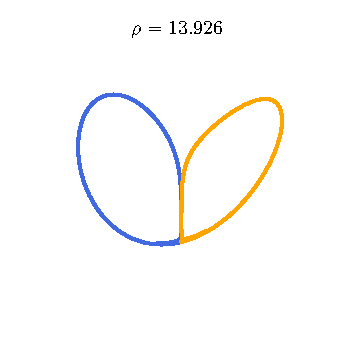
\includegraphics[width=.8\textwidth]{homoclinic_connection}
	\end{minipage}

	\vspace{1cm}
\end{frame}

\begin{frame}[t, c]{Lorenz system}{Pre-chaotic transients ($14 \leq \rho \leq 24$)}
	\centering
	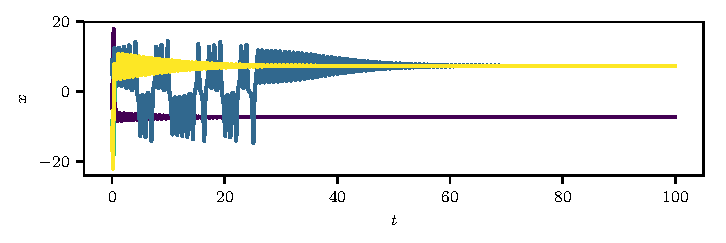
\includegraphics[width=.75\textwidth]{chaotic_transients_time_series}

	Pre-chaotic transient time series of $x(t)$ for $\rho=21$.
\end{frame}

\begin{frame}[t, c]{Lorenz system}{Pre-chaotic transients ($14 \leq \rho \leq 24$)}
	\begin{minipage}{.48\textwidth}
		For $14 \leq \rho \leq 24$, the system exhibits pre-chaotic transients.
		\begin{itemize}
			\item As $t \to \infty$, the system settles onto one of its stable equilibria.

			\bigskip

			\item It nonetheless exhibits some kind of \emph{sensitivity to initial conditions}.
		\end{itemize}
	\end{minipage}%
	\hfill
	\begin{minipage}{.48\textwidth}
		\centering
		
\includegraphics[width=.8\textwidth]{chaotic_transients_phase_space}
	\end{minipage}

	\vspace{1.5cm}
\end{frame}

\begin{frame}[t, c]{Lorenz system}{Subcritical Hopf bifucation at $\rho \simeq 24.74$}
	\begin{minipage}{.48\textwidth}
		\begin{itemize}
			\item A (subcritical) Hopf bifurcation occurs at $\rho \simeq 24.74$.

			\bigskip

			\item Trajectories escape from the symmetric fixed points and are repelled toward a distant attractor.
		\end{itemize}
	\end{minipage}%
	\hfill
	\begin{minipage}{.48\textwidth}
		\centering
		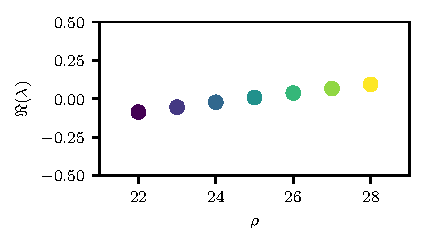
\includegraphics[width=.9\textwidth]{hopf_bifurcation_eigenvalue}
	\end{minipage}

	\vspace{1cm}
\end{frame}

\begin{frame}[t, c]{Lorenz system}{Chaos and strange attractors}
	\begin{minipage}{.48\textwidth}
		\centering
		
\includegraphics[width=.8\textwidth]{strange_attractor}
	\end{minipage}%
	\hfill
	\begin{minipage}{.48\textwidth}
		\alert{\textbf{Chaos}} is \emph{aperiodic long-term} behavior in a \emph{deterministic} system that exhibits \emph{sensitive dependence on initial conditions}.
	\end{minipage}

	\vspace{1cm}
\end{frame}

\begin{frame}[t, c]{Lorenz system}{Sensitivity to initial conditions}
	\centering
	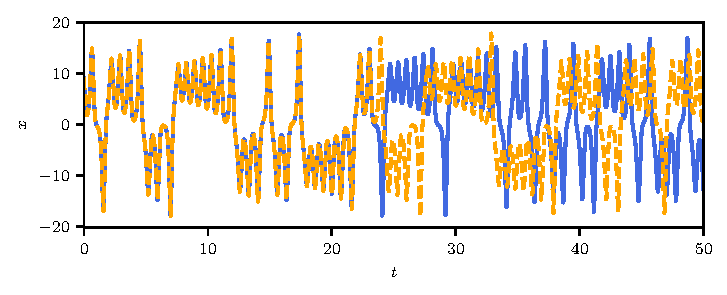
\includegraphics[width=.75\textwidth]{sensitivity_initial_conditions}

	\vspace{1cm}
\end{frame}

\begin{frame}[t, c]{Lorenz system}{Sensitivity to initial conditions}
	\begin{minipage}{.48\textwidth}
		\begin{itemize}
			\item Two nearby trajectories diverge exponentially rapidly from one another.

			\bigskip

			\item Prediction horizon hardly depends on how well the initial condition is characterized.

			\bigskip

			\item From a statistical point of view, the two trajectories nonetheless have the same properties.
		\end{itemize}
	\end{minipage}%
	\hfill
	\begin{minipage}{.48\textwidth}
		\centering
		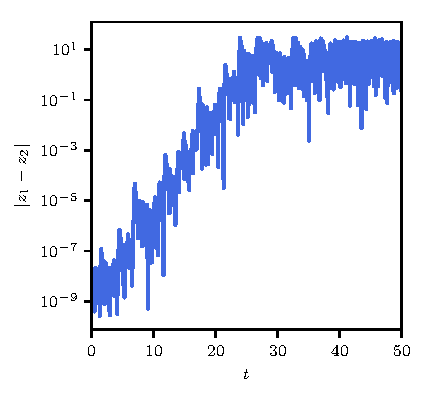
\includegraphics[width=.8\textwidth]{sensitivity_initial_conditions_bis}
	\end{minipage}

	\vspace{1cm}
\end{frame}

\begin{frame}[t, c]{Lorenz system}{Butterfly effect}
	\begin{quote}
		If a single flap of a butterfly's wing can be instrumental in generating a tornado, so all the previous and subsequent flaps of its wings, as can the flaps of the wings of millions of other butterflies, no to mention activities of innumerable more powerful creatures, including our own species. If a flap of a butterfly's wing can be instrumental in generating a tornado, it can equally well be instrumental in preventing a tornado.
	\end{quote}

	\begin{flushright}
		Conference by E. Lorenz, \emph{Predictability: does the flap of a \\ butterfly's wing in Brazil set off a tornado in Texas?}, 1972.
	\end{flushright}

	\vspace{1cm}
\end{frame}

\begin{frame}[t, c]{Lorenz system}{Bifurcation diagram}
	\centering
	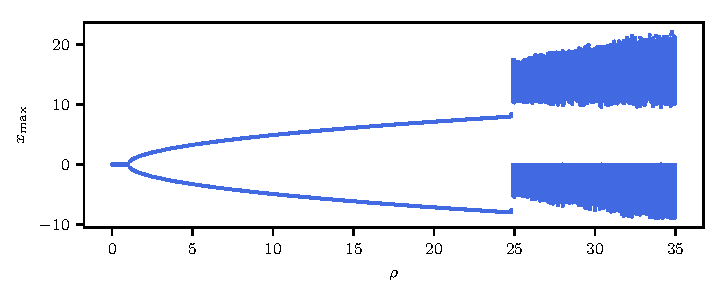
\includegraphics[width=.75\textwidth]{lorenz_bifurcation_diagram_1}

	Bifurcation diagram of the Lorenz system for $0 \leq \rho \leq 35$.
	\vspace{1cm}
\end{frame}

\begin{frame}[t, c]{}
	\centering
	\vspace{1cm}

	{\Large \textbf{On the importance of chaos in science}}

	\bigskip

	{\textgre{\textbf{A (very) brief history}}}

\end{frame}

\begin{frame}[t, c]{On the importance of chaos in science}{A (very) brief history}
	\begin{itemize}
		\item \alert{\textbf{1814}}: Laplacian determinism.

		\bigskip

		\item \alert{\textbf{1820 -- 1868}}: Cauchy-Lipschitz theorem on the existence and uniqueness of solutions to ordinary differential equations.

		\bigskip

		\item \alert{\textbf{1888}}: Poincaré and the \emph{three bodies problem}. First example of sensitivity to initial conditions.
	\end{itemize}

	\vspace{1cm}
\end{frame}

\begin{frame}[t, c]{On the importance of chaos in science}{Laplacian determinism}
	\begin{quote}
		Nous devons [...] envisager l'état présent de l'univers comme l'effet de son état antérieur, et comme la cause de celui qui va suivre. Une intelligence qui pour un instant donné connaîtrait toutes les forces dont la nature est animée et la situation respective des êtres qui la composent [...] embrasserait dans la même formule les mouvements des plus grands corps de l'univers et ceux du plus léger atome : rien ne serait incertain pour elle, et l'avenir comme le passé serait présent à ses yeux.
	\end{quote}

	\begin{flushright}
		\emph{Essai philosophique sur les probabilités}, \\ Pierre SImon de Laplace, 1814.
	\end{flushright}
\end{frame}

\begin{frame}[t, c]{On the importance of chaos in science}{Poincaré and the sensitivity to initial conditions}
	\begin{quote}
		Une cause très petite, qui nous échappe, détermine un effet considérable que nous ne pouvons pas ne pas voir, et alors nous disons que cet effet est dû au hasard. Si nous connaissions exactement les lois de la nature et la situation de l'univers à l'instant initial, nous pourrions prédire exactement la situation de ce même univers à un instant ultérieur. Mais, lors même que les lois naturelles n'auraient plus de secret pour nous, nous ne pourrions connaître la situation qu'approximativement. Si cela nous permet de prévoir la situation ultérieure avec la même approximation, c'est tout ce qu'il nous faut, nous disons que le phénomène a été prévu, qu'il est régi par des lois ; mais il n'en est pas toujours ainsi, il peut arriver que de petites différences dans les conditions initiales en engendrent de très grandes dans les phénomènes finaux ; une petite erreur sur les premières produirait une erreur énorme sur les derniers. La prédiction devient impossible et nous avons le phénomène fortuit.
	\end{quote}

	\begin{flushright}
		\emph{Calcul des probabilités},\\ Henri Poincaré, 1912.
	\end{flushright}

	\vspace{1cm}
\end{frame}

\begin{frame}[t, c]{On the importance of chaos in science}{A (very) brief history}
	\begin{itemize}
		\item \alert{\textbf{1963}}: Edward Lorenz introduced his simplified model of thermal convection.

		\bigskip

		\item \alert{\textbf{1975}}: Tien-Yien Li and James A. Yorke coined the term \emph{deterministic chaos}.

		\bigskip

		\item \alert{\textbf{1976}}: Introduction of the R\"ossler model.

		\bigskip

		\item \alert{\textbf{1971}}: Ruelle \& Takens introduced the concept of \emph{strange attractors}.
	\end{itemize}

	\vspace{1cm}
\end{frame}

\end{document}
